\chapter{Arquitetura do Software}

%% ─────────────────────────────────────────────
\section{Abordagem de Descrição Arquitetural}

A descrição arquitetural do Sistema de Gestão de Clínica (SGC) segue a norma \textbf{ISO/IEC/IEEE 42010:2022}, que define um framework conceitual para a expressão, comunicação e revisão de arquiteturas de sistemas de software. Segundo essa norma, a descrição arquitetural deve registrar as decisões de design que satisfazem os concerns das partes interessadas, organizando-as em \textit{viewpoints} e \textit{views} com seus respectivos modelos.

Adicionalmente, a estrutura da descrição segue o modelo de maturidade \textbf{ArchCaMo} (\textit{Architecture Completeness Model}), que permite avaliar o grau de completude e rastreabilidade dos artefatos arquiteturais. Cada seção deste capítulo corresponde a elementos do ArchCaMo, garantindo aderência ao nível de completude esperado para projetos de software clínico.

A elaboração das \textit{views} e modelos considera também a norma \textbf{ISO/IEC/IEEE 42020:2019}, especialmente a atividade de elaboração arquitetural, que orienta como arquiteturas devem ser criadas, analisadas e avaliadas de forma sistemática no contexto do sistema de interesse.

%% ─────────────────────────────────────────────
\section{Sistema de Interesse, Ambiente e Escopo Arquitetural}

O \textbf{sistema de interesse} é o SGC --- um sistema de software para gestão integral de clínicas de saúde, compreendendo os módulos de agendamento, prontuário eletrônico, farmácia clínica, faturamento, controle de acesso e gestão de recursos físicos.

O \textbf{ambiente} é composto por: clínicas de pequeno e médio porte, usuários internos (recepcionistas, médicos, farmacêuticos, administradores), operadores de convênios e plataforma em nuvem com acesso via navegador web.

O \textbf{escopo arquitetural} abrange:
\begin{itemize}
    \item A estrutura interna do sistema e seus componentes de software;
    \item As interações entre os módulos e a camada de persistência;
    \item Os mecanismos de segurança, auditoria e controle de acesso;
    \item A estratégia de implantação em ambiente de nuvem.
\end{itemize}

Estão \textbf{fora do escopo}: integrações com sistemas de saúde externos (e.g., TISS, HL7), equipamentos médicos, aplicativos móveis para pacientes e módulos de telemedicina.

%% ─────────────────────────────────────────────
\section{Stakeholders e Concerns Arquiteturais}
 
\subsection{Stakeholders Arquiteturais}
 
Os stakeholders foram decompostos em perfis atômicos, cada um com responsabilidades
e interesses distintos sobre a arquitetura. A \autoref{tab:stakeholders-arquitetura}
apresenta os onze perfis identificados.
 
\begin{table}[H]
\caption{Stakeholders arquiteturais e concerns associados.}
\label{tab:stakeholders-arquitetura}
\centering
\small
\begin{tabularx}{\textwidth}{|l|l|X|l|}
\hline
\textbf{ID} & \textbf{Stakeholder} & \textbf{Responsabilidade principal} & \textbf{Concerns} \\
\hline
S1  & Desenvolvedor front-end     & Implementa a interface React e consome a API REST & C7, C8, C9, C11 \\
\hline
S2  & Desenvolvedor back-end      & Implementa regras de negócio, endpoints e transações & C4, C7, C8, C11 \\
\hline
S3  & Administrador de sistemas   & Configura usuários, perfis e audita operações sensíveis & C1, C5, C6 \\
\hline
S4  & Médico / Clínico            & Registra atendimentos, evolução clínica e prescrições & C2, C4, C9 \\
\hline
S5  & Recepcionista               & Gerencia agenda de consultas e cadastros de pacientes & C2, C4, C9 \\
\hline
S6  & Farmacêutico                & Realiza dispensações e controla estoque de medicamentos & C4, C5, C10 \\
\hline
S7  & Financeiro                  & Gera cobranças, confere convênios e emite comprovantes & C4, C9, C10 \\
\hline
S8  & DevOps     & Mantém infraestrutura, monitora serviços e executa deploys & C3, C10, C12 \\
\hline
S9  & Responsável pela conformidade (DPO) & Verifica aderência à LGPD e conduz auditorias & C5, C6, C1 \\
\hline
S10 & Paciente                    & Recebe confirmações de consulta e comprovantes & C2, C9 \\
\hline
S11 & Gestor da clínica           & Acompanha relatórios financeiros e operacionais & C5, C9, C12 \\
\hline
\end{tabularx}
\end{table}
 
\subsection{Concerns Arquiteturais}
 
Os \textit{concerns} representam os interesses, objetivos e restrições que a
arquitetura deve satisfazer. Para cada concern, descreve-se o interesse geral e,
em seguida, como cada stakeholder o interpreta de forma particular.
 
\begin{longtable}{|l|l|p{9.5cm}|}
\caption{Concerns arquiteturais do SGC com perspectiva por stakeholder.}
\label{tab:concerns-arquitetura} \\
\hline
\textbf{ID} & \textbf{Concern} & \textbf{Descrição geral e perspectiva por stakeholder} \\
\hline
\endfirsthead
\hline
\textbf{ID} & \textbf{Concern} & \textbf{Descrição geral e perspectiva por stakeholder} \\
\hline
\endhead
\hline
\endfoot
 
C1 & Controle de acesso e segurança &
Somente usuários autorizados executam operações sensíveis; autenticação robusta e RBAC granular.
\newline\textbf{S3 (Admin. sistemas):} precisa criar, inativar e auditar contas sem expor o sistema a escalada de privilégios.
\newline\textbf{S9 (DPO):} exige que nenhum dado de paciente seja acessível a perfis não autorizados, com rastreio de cada acesso. \\
\hline
C2 & Desempenho e responsividade &
Tempos de resposta aceitáveis nas operações cotidianas.
\newline\textbf{S4 (Médico):} espera que a abertura do prontuário e o registro de evolução respondam em menos de dois segundos durante o atendimento.
\newline\textbf{S5 (Recepcionista):} precisa que o calendário de agendamentos carregue sem atraso perceptível ao receber pacientes em fila.
\newline\textbf{S10 (Paciente):} aguarda confirmação de consulta imediata no balcão ou por canal digital. \\
\hline
C3 & Disponibilidade e continuidade &
Sistema operacional mesmo em falhas parciais; recuperação e backups automáticos.
\newline\textbf{S8 (DevOps):} requer que falhas em um contêiner não derrubem o sistema inteiro e que backups sejam verificáveis. \\
\hline
C4 & Integridade transacional &
Atomicidade nas operações críticas: nenhuma escrita parcial deve ser persistida.
\newline\textbf{S2 (Dev. back-end):} implementa transações ACID nos serviços de agendamento, dispensação e faturamento.
\newline\textbf{S4 (Médico):} o prontuário deve refletir exatamente o que foi salvo; uma falha não pode corromper o registro clínico.
\newline\textbf{S5 (Recepcionista):} dois recepcionistas não podem confirmar o mesmo slot simultaneamente.
\newline\textbf{S6 (Farmacêutico):} a baixa de estoque e o registro de dispensação devem ocorrer atomicamente.
\newline\textbf{S7 (Financeiro):} a cobrança e os itens de conta devem ser gerados ou revertidos juntos. \\
\hline
C5 & Rastreabilidade e auditoria &
Registro completo e imutável de operações para auditoria, conformidade e investigação.
\newline\textbf{S3 (Admin. sistemas):} precisa consultar quem alterou permissões ou inativou cadastros.
\newline\textbf{S6 (Farmacêutico):} toda dispensação deve ter rastro de lote, quantidade e responsável.
\newline\textbf{S9 (DPO):} os logs de acesso a dados pessoais devem ser preservados pelo período legal.
\newline\textbf{S11 (Gestor):} relatórios de operações realizadas por período devem ser geráveis a qualquer momento. \\
\hline
C6 & Conformidade com LGPD &
Proteção de dados pessoais e sensíveis de pacientes conforme a Lei 13.709/2018.
\newline\textbf{S3 (Admin. sistemas):} garante que dados só sejam acessados por usuários com finalidade justificada.
\newline\textbf{S9 (DPO):} exige criptografia em repouso para arquivos clínicos, anonimização em relatórios e política de retenção de dados. \\
\hline
C7 & Modularidade e manutenibilidade &
Módulos coesos e de baixo acoplamento, facilitando evoluções e manutenções independentes.
\newline\textbf{S1 (Dev. front-end):} quer consumir contratos de API estáveis sem depender de detalhes do back-end.
\newline\textbf{S2 (Dev. back-end):} quer alterar a lógica de farmácia sem risco de quebrar o módulo de agendamento. \\
\hline
C8 & Interoperabilidade entre módulos &
Comunicação padronizada entre módulos internos via interfaces bem definidas.
\newline\textbf{S1 (Dev. front-end):} consome a API via contrato OpenAPI; mudanças de implementação não devem exigir retrabalho no cliente.
\newline\textbf{S2 (Dev. back-end):} os módulos de domínio se comunicam por interfaces de serviço; nenhum módulo acessa diretamente o repositório de outro. \\
\hline
C9 & Experiência e usabilidade &
Interface intuitiva e responsiva, adequada ao fluxo de trabalho clínico.
\newline\textbf{S4 (Médico):} o formulário de evolução deve ser rápido de preencher sem alternar entre múltiplas telas.
\newline\textbf{S5 (Recepcionista):} o calendário deve permitir criar e remarcar consultas com poucos cliques.
\newline\textbf{S7 (Financeiro):} as telas de cobrança devem exibir os valores calculados antes de confirmar.
\newline\textbf{S10 (Paciente):} confirmações e comprovantes devem ser legíveis e imediatos.
\newline\textbf{S11 (Gestor):} painéis de relatório devem ser compreensíveis sem treinamento técnico. \\
\hline
C10 & Persistência e consistência &
Durabilidade dos dados e consistência entre banco relacional e storage de arquivos clínicos.
\newline\textbf{S6 (Farmacêutico):} os saldos de estoque devem refletir cada dispensação em tempo real.
\newline\textbf{S7 (Financeiro):} os valores faturados não podem divergir do que está registrado nas cobranças.
\newline\textbf{S8 (DevOps):} backups do banco e do storage devem ser sincronizados e restauráveis de forma consistente. \\
\hline
C11 & Testabilidade e qualidade &
Código estruturado para testes unitários, de integração e regressão automatizados.
\newline\textbf{S1 (Dev. front-end):} componentes React devem ser testáveis isoladamente com dados mockados.
\newline\textbf{S2 (Dev. back-end):} serviços de domínio devem ser injetáveis e testáveis sem depender do banco real. \\
\hline
C12 & Operação e implantação &
Implantação automatizada, monitoramento contínuo e rollback seguro em nuvem.
\newline\textbf{S8 (DevOps):} o pipeline CI/CD deve implantar novas versões sem downtime e permitir rollback em um comando.
\newline\textbf{S11 (Gestor):} precisa saber o status operacional do sistema sem depender da equipe técnica para obter essa informação. \\
\hline
 
\end{longtable}
 
\subsection{Matriz Concern--Stakeholder}
 
A \autoref{tab:matriz-concern-stakeholder} relaciona cada concern com os stakeholders
afetados, utilizando \textbf{P} (primário) e \textbf{S} (secundário).
 
\begin{table}[H]
\caption{Matriz Concern--Stakeholder.}
\label{tab:matriz-concern-stakeholder}
\centering
\footnotesize
\setlength{\tabcolsep}{4pt}
\begin{tabularx}{\textwidth}{|X|*{11}{>{\centering\arraybackslash}p{0.85cm}|}}
\hline
\textbf{Concern}
  & \textbf{S1} & \textbf{S2} & \textbf{S3} & \textbf{S4}
  & \textbf{S5} & \textbf{S6} & \textbf{S7} & \textbf{S8}
  & \textbf{S9} & \textbf{S10} & \textbf{S11} \\
\hline
C1 -- Acesso/Segurança     & -- & -- & P  & S  & S  & S  & --  & S  & P  & --  & -- \\
C2 -- Desempenho           & S  & S  & -- & P  & P  & S  & --  & S  & -- & S   & -- \\
C3 -- Disponibilidade      & -- & S  & -- & -- & -- & -- & --  & P  & -- & --  & S  \\
C4 -- Integridade transac. & -- & P  & -- & P  & P  & P  & P   & -- & S  & --  & -- \\
C5 -- Auditoria            & -- & S  & P  & -- & -- & P  & --  & -- & P  & --  & S  \\
C6 -- LGPD                 & -- & S  & P  & S  & -- & -- & --  & S  & P  & --  & -- \\
C7 -- Modularidade         & P  & P  & -- & -- & -- & -- & --  & S  & -- & --  & -- \\
C8 -- Interoperab.         & P  & P  & -- & S  & S  & S  & S   & S  & -- & --  & -- \\
C9 -- Usabilidade          & S  & -- & -- & P  & P  & S  & P   & -- & -- & P   & S  \\
C10 -- Persistência        & -- & S  & -- & -- & -- & P  & P   & P  & -- & --  & -- \\
C11 -- Testabilidade       & P  & P  & -- & -- & -- & -- & --  & S  & -- & --  & -- \\
C12 -- Implantação         & -- & S  & -- & -- & -- & -- & --  & P  & -- & --  & S  \\
\hline
\end{tabularx}
\end{table}














%% ─────────────────────────────────────────────
\section{Viewpoints e Views Arquiteturais}

Seguindo a ISO 42010, foram definidos seis \textit{viewpoints} que orientam a construção das \textit{views} arquiteturais do SGC. A \autoref{tab:viewpoints-visoes} apresenta o mapeamento entre viewpoints, views, concerns abordados e modelos produzidos.

\begin{table}[htbp]
\caption{Viewpoints, views, concerns e modelos arquiteturais.}
\label{tab:viewpoints-visoes}
\centering
\small
\begin{tabularx}{\textwidth}{|l|l|l|X|l|}
\hline
\textbf{Viewpoint} & \textbf{View} & \textbf{Model Kind} & \textbf{Concerns} & \textbf{Modelo} \\
\hline
Cenários         & V1 & UML Sequence Diagram     & C1, C4, C5, C7  & M-V1-01 \\
Lógico           & V2 & UML Component     & C7, C8, C10     & M-V2-01 \\
Processos        & V3 & UML Component     & C2, C4, C5, C8  & M-V3-01 \\
Desenvolvimento  & V4 & UML Component (camadas) & C7, C8, C11 & M-V4-01 \\
Implantação      & V5 & UML Deployment    & C3, C10, C12    & M-V5-01 \\
Segurança        & V6 & UML Component     & C1, C5, C6      & M-V6-01 \\
\hline
\end{tabularx}
\end{table}

%% ─────────────────────────────────────────────
\section{Visão de Cenários}
 
A visão de cenários é a visão ``+1'' do modelo 4+1: ela não introduz novos artefatos de
implementação, mas valida que os elementos das outras quatro visões trabalham em conjunto
para realizar os fluxos de negócio críticos do sistema. Os cenários foram selecionados com
base nos casos de uso de maior risco e impacto operacional, conforme a
\autoref{tab:cenarios-criticos}.
 
\begin{table}[htbp]
\caption{Cenários críticos usados para validar a arquitetura.}
\label{tab:cenarios-criticos}
\centering
\small
\begin{tabularx}{\textwidth}{|l|X|l|l|}
\hline
\textbf{ID} & \textbf{Cenário} & \textbf{Concerns} & \textbf{Modelo} \\
\hline
CN-01 & Agendamento de consulta com validação de disponibilidade e auditoria & C1, C4, C5, C7 & M-V1-01 \\
CN-02 & Dispensação de medicamento com validação de prescrição e baixa de estoque & C2, C4, C5, C8 & -- \\
CN-03 & Autenticação e autorização RBAC na entrada do sistema & C1, C6 & M-V6-01 \\
\hline
\end{tabularx}
\end{table}
 
\subsection{Cenário CN-01 — Agendamento de Consulta}
 
O cenário de agendamento ilustra como as quatro visões arquiteturais colaboram para
executar um dos fluxos de maior frequência e impacto transacional do SGC.
 
\begin{enumerate}
    \item \textbf{(Visão Física)} A Recepcionista acessa o SGC pelo navegador em seu
    computador na rede interna da clínica. A requisição trafega via HTTPS até o contêiner
    de front-end hospedado na DigitalOcean.
 
    \item \textbf{(Visão de Desenvolvimento)} A interface React, pertencente à camada de
    Apresentação, envia uma chamada à camada de API REST. A ação ativa o
    \texttt{AgendamentoController}, localizado no Módulo de Agenda e Atendimento da camada
    de Aplicação.
 
    \item \textbf{(Visão Lógica)} O Módulo de Agenda consulta o Módulo de Controle de
    Acesso para verificar se a Recepcionista possui a permissão
    \texttt{agenda:escrever}. Confirmada a autorização, o módulo aciona o serviço de
    domínio responsável pela validação de disponibilidade do slot horário.
 
    \item \textbf{(Visão de Processos)} A API realiza uma transação atômica no banco
    PostgreSQL (Supabase): bloqueia o slot, registra a consulta e grava o evento de
    auditoria em uma única operação, garantindo que dois usuários simultâneos não
    consigam reservar o mesmo horário.
 
    \item Concluída a transação, a API retorna confirmação ao front-end, que exibe a
    consulta registrada na agenda.
\end{enumerate}
 
Esse cenário demonstra a integração entre a camada de apresentação (V4), o módulo lógico
de agendamento (V2), o mecanismo transacional de rede (V3) e o nó de banco de dados em
nuvem (V5), validando as correspondências CO-01, CO-03, CO-04 e CO-05.
 


%% ─────────────────────────────────────────────
\section{Visão Lógica}

A visão lógica decompõe o sistema em componentes funcionais coesos, evidenciando as responsabilidades de cada módulo e suas dependências. Essa view endereça os concerns de modularidade (C7), interoperabilidade (C8) e persistência (C10).

\subsection{Modelo M-V2-01 -- Componentes Lógicos}

O modelo M-V2-01 apresenta a decomposição funcional do SGC em componentes lógicos organizados em pacotes. A camada de \textit{Módulos de Domínio} concentra as regras de negócio clínico e administrativo, enquanto a camada de \textit{API REST} define a interface entre a interface web e o núcleo do sistema.

\begin{figure}[H]
\centering
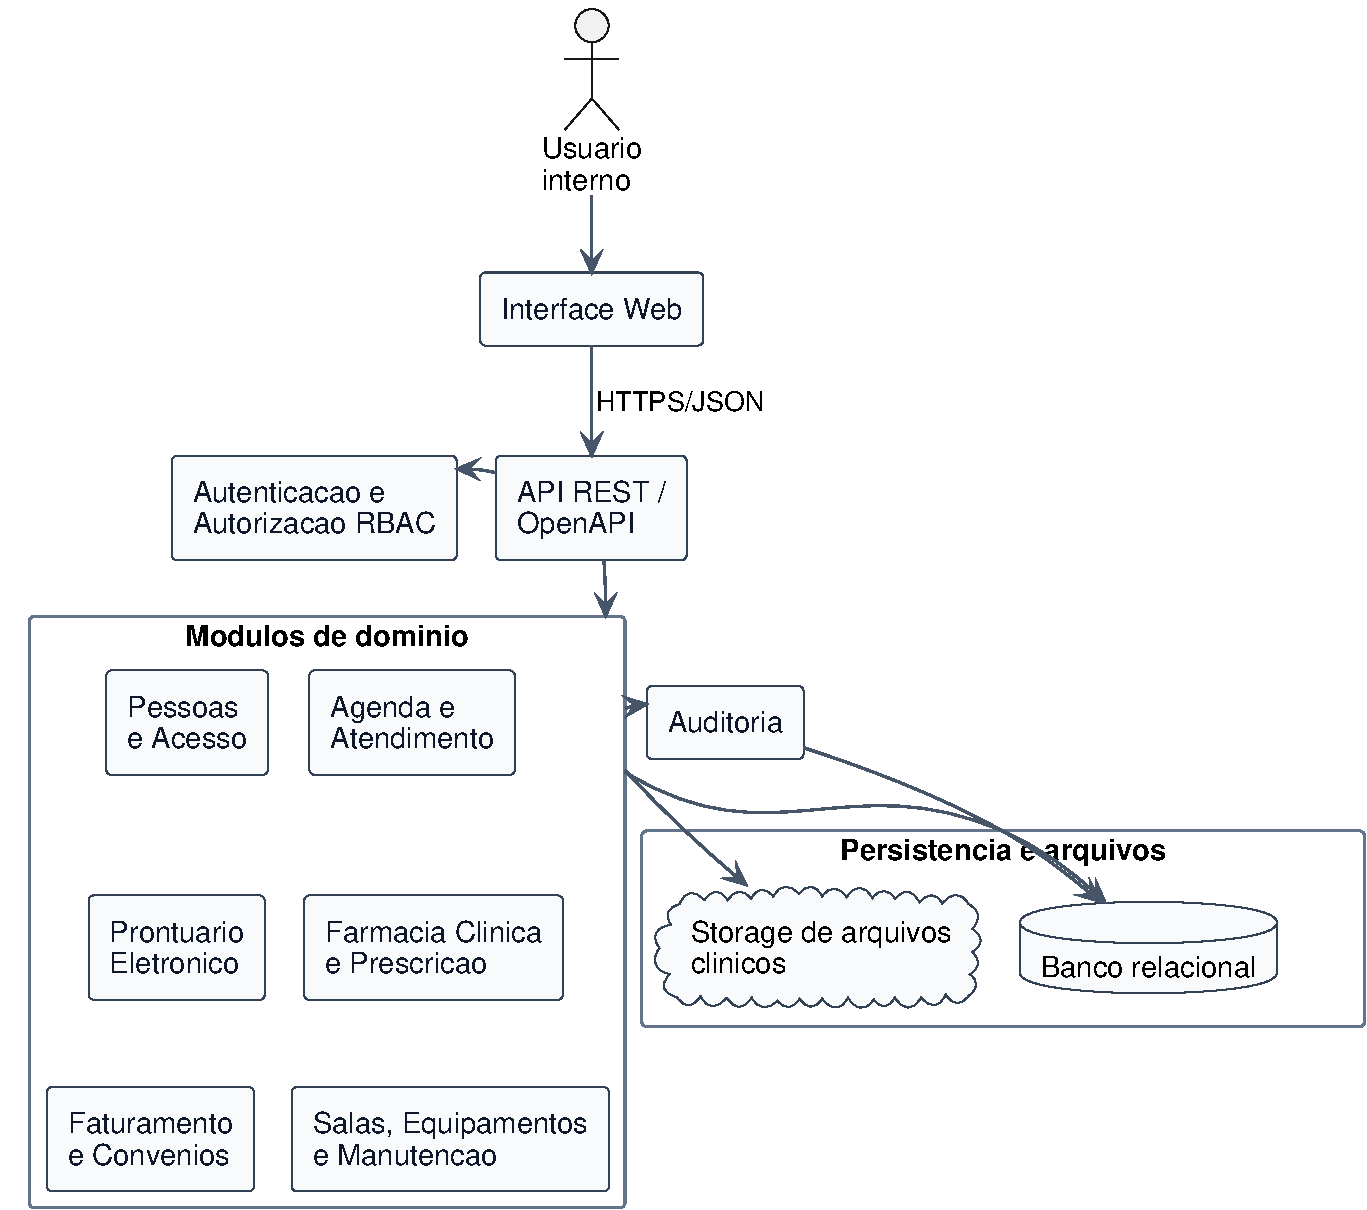
\includegraphics[width=\textwidth,height=0.50\textheight,keepaspectratio]{Imagens/arquitetura/M-V2-01-componentes-logicos}
\caption{Modelo M-V2-01 -- Componentes lógicos do Sistema de Gestão de Clínica.}
\label{fig:m-v2-01-componentes-logicos}
\end{figure}



%% ─────────────────────────────────────────────
\section{Visão de Processos}
 
A visão de processos descreve o comportamento dinâmico e de execução do SGC, tratando
os concerns de desempenho (C2), integridade transacional (C4), rastreabilidade (C5) e
interoperabilidade entre módulos (C8). Ela responde à pergunta: \textit{quais processos
existem em execução e como se comunicam?}
 
\subsection{Modelo de Execução — Arquitetura Cliente/Servidor}
 
O SGC opera segundo uma arquitetura \textbf{Cliente/Servidor} com três processos
principais em execução:
 
\begin{itemize}
    \item \textbf{Processo do Cliente (Navegador/React):} executa no dispositivo do
    usuário e é responsável pela renderização da interface e pelo envio de requisições.
 
    \item \textbf{Processo da API (FastAPI):} executa em contêiner na nuvem e concentra
    toda a lógica de negócio, autenticação, autorização e orquestração dos módulos de
    domínio.
 
    \item \textbf{Processo do Banco de Dados (PostgreSQL/Supabase):} executa como serviço
    gerenciado e é o único responsável pela persistência e atomicidade das transações.
\end{itemize}
 
A comunicação entre o Cliente e a API é \textbf{síncrona}, realizada via
\texttt{HTTPS/REST} com contrato \texttt{JSON}. A comunicação entre a API e o banco é
\textbf{transacional}, utilizando \texttt{SQL} com suporte a transações ACID — garantindo
que operações críticas como agendamento e dispensação sejam atômicas e não gerem estados
inconsistentes em caso de falha parcial.
 
\subsection{Modelo M-V3-01 — Fluxo de Processos}
 
A \autoref{fig:m-v3-01-processos} apresenta o diagrama de componentes da visão de
processos, evidenciando os três processos em execução e os protocolos de comunicação
entre eles.
 
\begin{figure}[htbp]
\centering
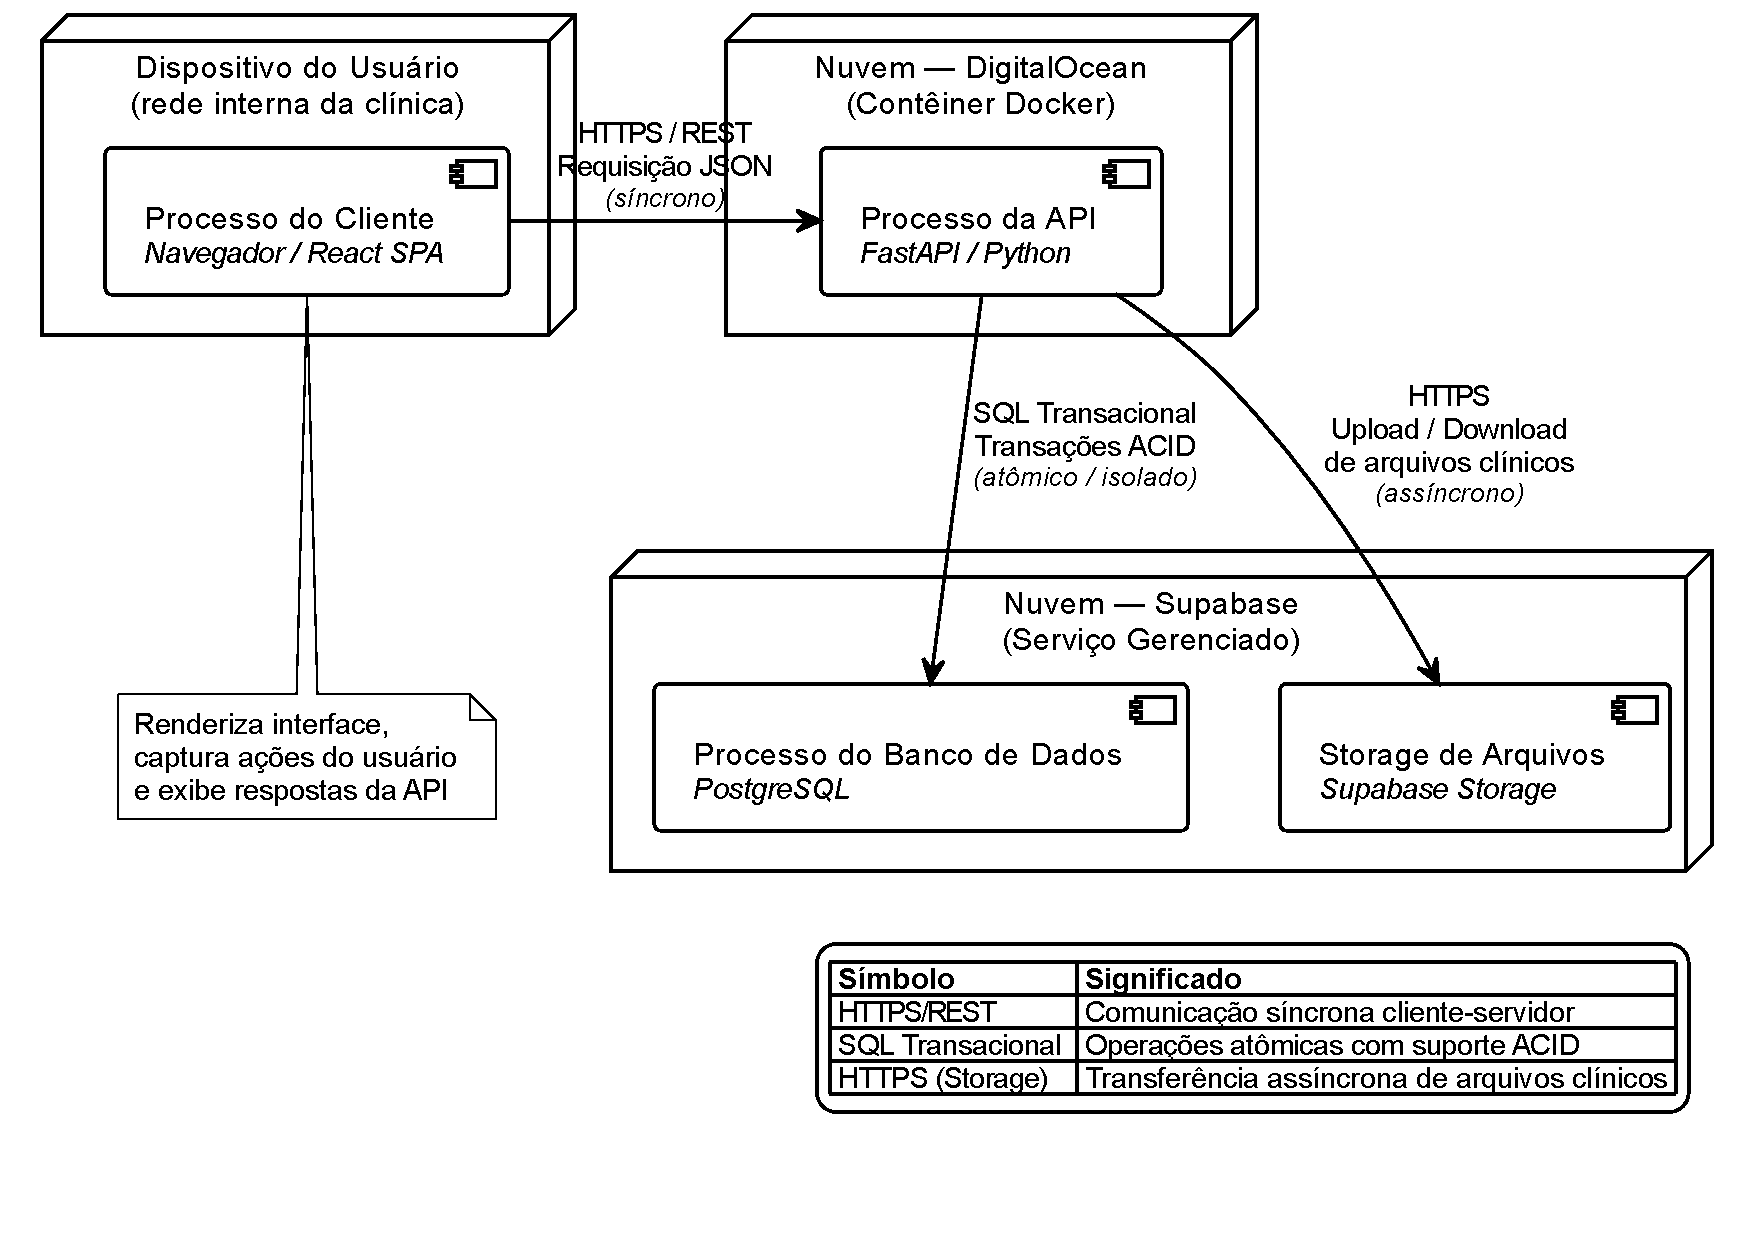
\includegraphics[width=0.85\textwidth,keepaspectratio]{Imagens/arquitetura/M-V3-01-processos.pdf}
\caption{Modelo M-V3-01 — Fluxo de processos e comunicação entre camadas de execução.}
\label{fig:m-v3-01-processos}
\end{figure}
 
\subsection{Controle de Concorrência}
 
Uma consequência direta da arquitetura de processos é o tratamento de concorrência. Quando
dois usuários tentam agendar o mesmo slot horário simultaneamente, a sequência abaixo
garante a integridade dos dados:
 
\begin{enumerate}
    \item Ambos os processos clientes enviam requisições \texttt{POST /consultas} à API
    de forma concorrente.
    \item A API encaminha as duas operações ao banco, que as executa dentro de
    transações isoladas (\textit{serializable isolation}).
    \item O banco concede o bloqueio à primeira transação a chegar; a segunda recebe
    uma exceção de conflito.
    \item A API captura o conflito e retorna \texttt{HTTP 409 Conflict} ao segundo
    cliente, que exibe a mensagem de horário indisponível.
\end{enumerate}
 
Esse mecanismo satisfaz diretamente o concern C4 (integridade transacional) e está
alinhado à decisão arquitetural DA06.
 









%% ─────────────────────────────────────────────
\section{Visão de Desenvolvimento}

A visão de desenvolvimento organiza o sistema em camadas lógicas de responsabilidade, facilitando a compreensão da estrutura de código e suportando os concerns de modularidade (C7), interoperabilidade (C8) e testabilidade (C11).

\subsection{Modelo M-V4-01 -- Camadas}

O modelo M-V4-01 apresenta a organização em camadas do SGC, seguindo o padrão \textit{Layered Architecture}. Cada camada possui responsabilidades bem delimitadas e se comunica somente com a camada adjacente, exceto a camada de Domínio que acessa a Infraestrutura compartilhada para persistência.

\begin{figure}[htbp]
\centering
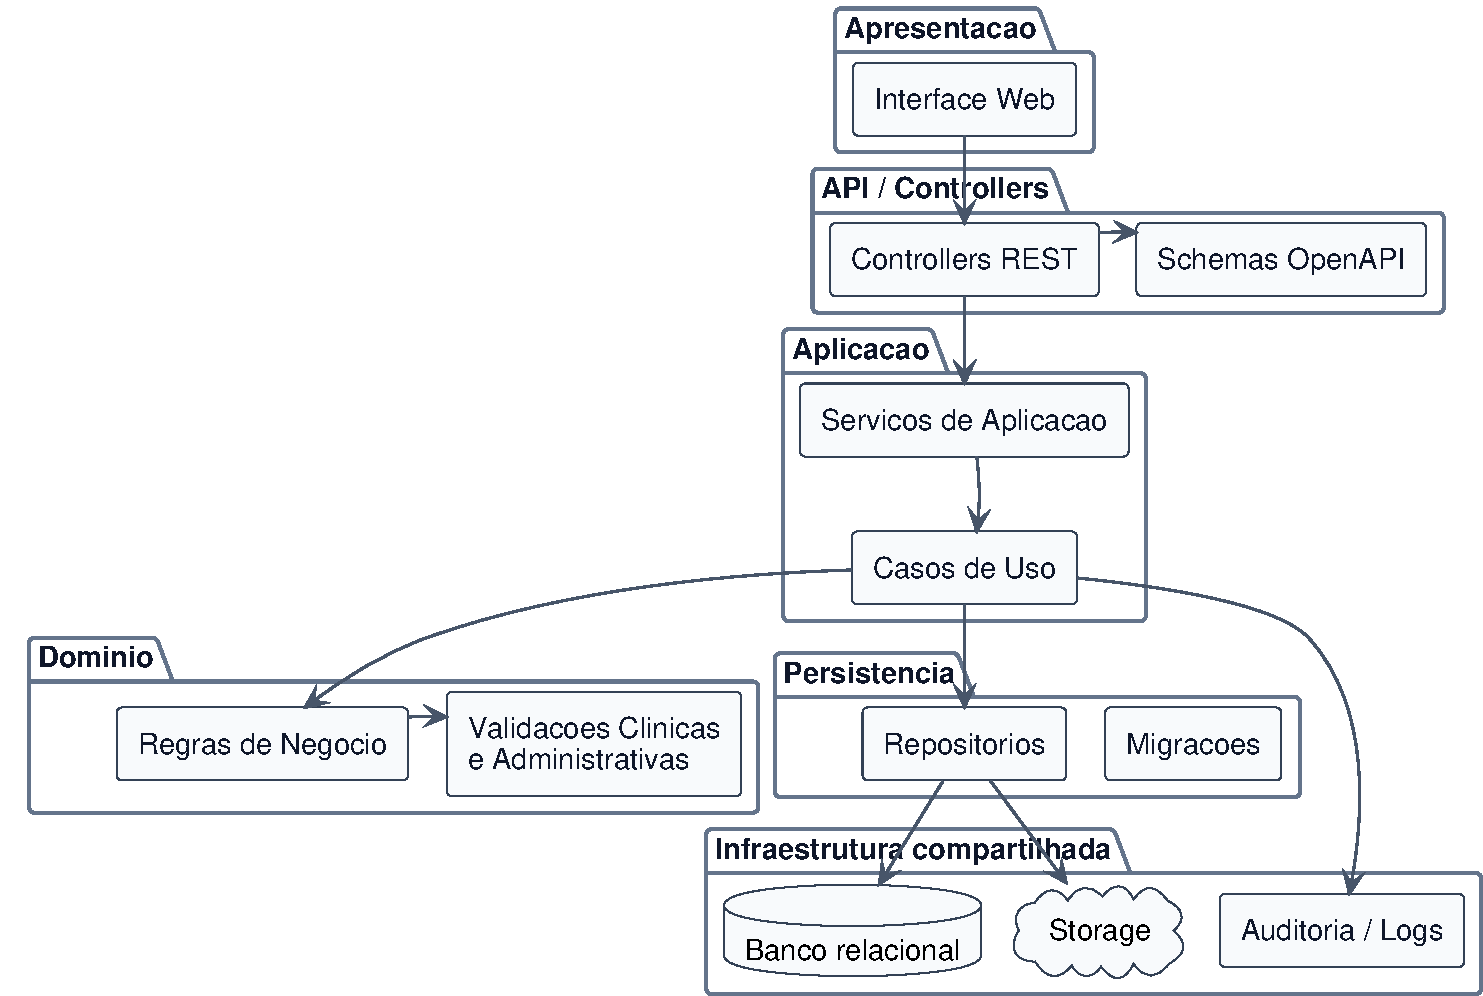
\includegraphics[width=1.0\textwidth,height=0.80\textheight,keepaspectratio]{Imagens/arquitetura/M-V4-01-camadas}
\caption{Modelo M-V4-01 -- Camadas lógicas da aplicação.}
\label{fig:m-v4-01-camadas}
\end{figure}

%% ─────────────────────────────────────────────
\section{Visão Física ou de Implantação}

A visão de implantação descreve a distribuição dos artefatos de software nos nós de execução, endereçando os concerns de disponibilidade (C3), persistência (C10) e operação (C12).

\subsection{Modelo M-V5-01 -- Implantação}

O modelo M-V5-01 mapeia os contêineres de execução e serviços de infraestrutura utilizados pelo SGC. A solução adota plataforma em nuvem com ambientes separados de produção e homologação, pipeline de CI/CD automatizado e serviços gerenciados de banco de dados e armazenamento via Supabase.

\begin{figure}[H]
\centering
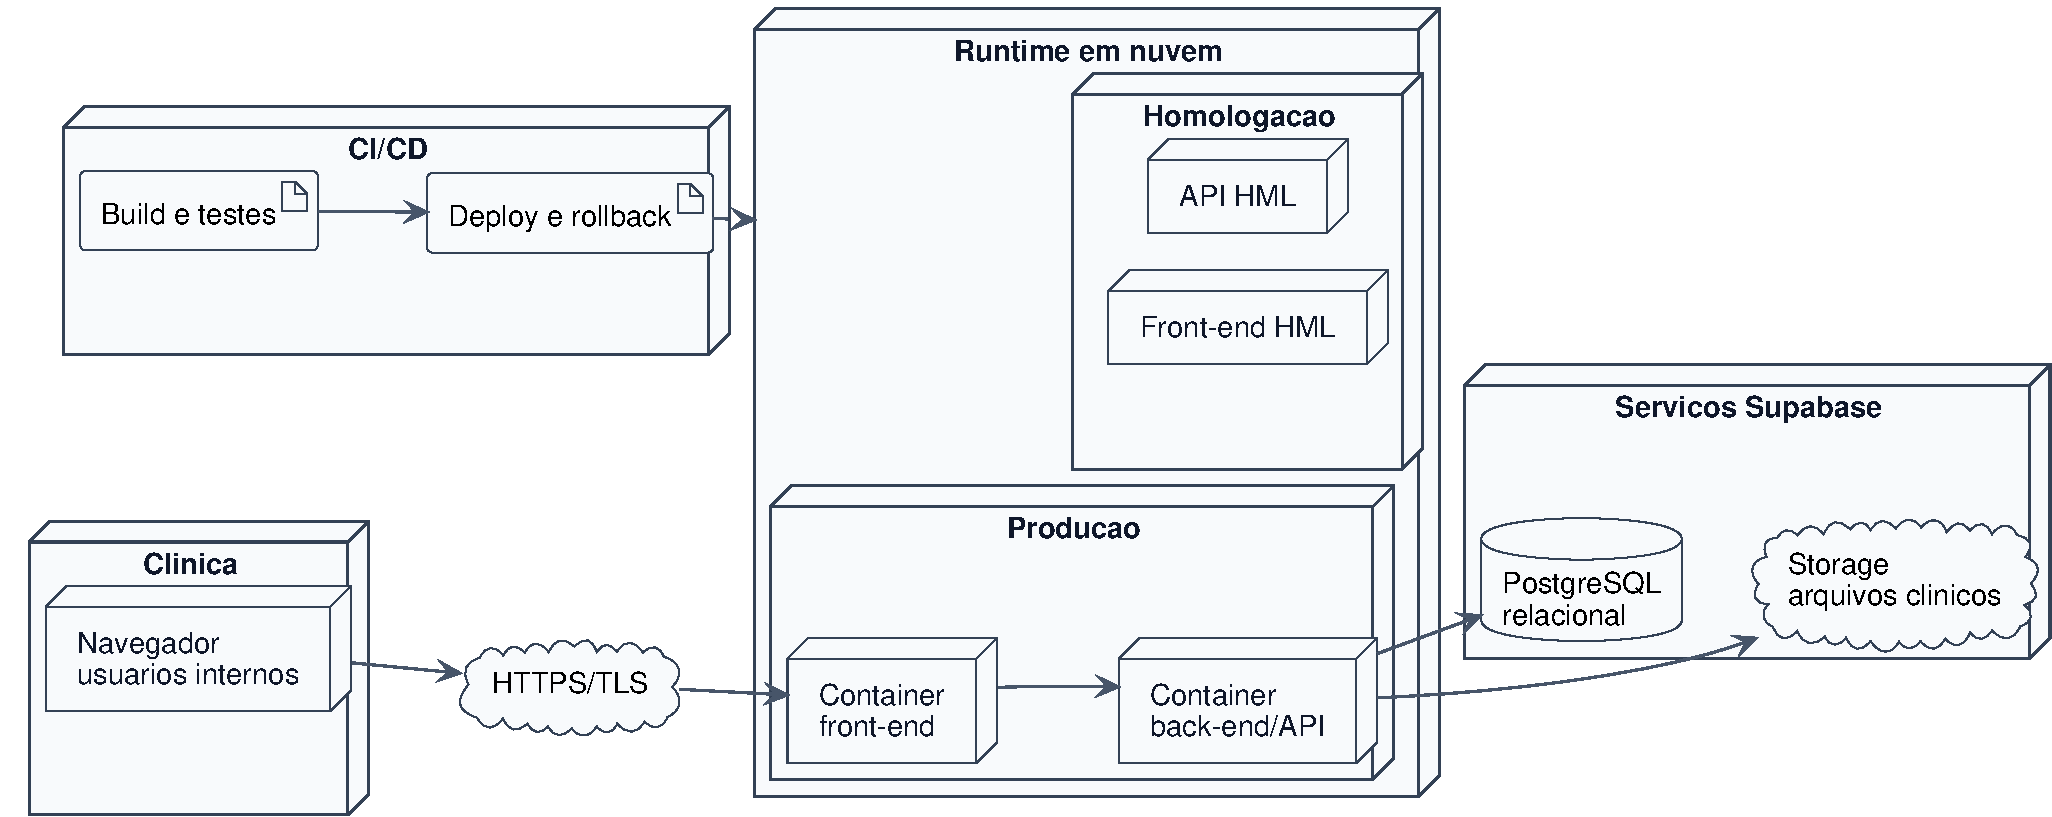
\includegraphics[width=0.82\textwidth,height=0.28\textheight,keepaspectratio]{Imagens/arquitetura/M-V5-01-implantacao}
\caption{Modelo M-V5-01 -- Implantação do Sistema de Gestão de Clínica.}
\label{fig:m-v5-01-implantacao}
\end{figure}
\vspace{-0.8em}

%% ─────────────────────────────────────────────
\section{Visão de Segurança e Conformidade}

A visão de segurança aborda os mecanismos de proteção dos dados e controle de acesso do SGC, endereçando os concerns de segurança (C1), auditoria (C5) e conformidade com LGPD (C6). O controle de acesso é implementado por meio de RBAC (\textit{Role-Based Access Control}), com papéis mapeados às funcionalidades do sistema.

A \autoref{tab:rbac-resumido} apresenta a matriz RBAC resumida com os principais papéis e permissões.

\begin{table}[htbp]
\caption{Matriz RBAC resumida.}
\label{tab:rbac-resumido}
\centering
\small
\begin{tabular}{|l|c|c|c|c|c|}
\hline
\textbf{Funcionalidade} & \textbf{Admin} & \textbf{Médico} & \textbf{Recep.} & \textbf{Farm.} & \textbf{TI} \\
\hline
Cadastro de pacientes      & \checkmark & -- & \checkmark & -- & -- \\
Agendamento de consultas   & \checkmark & \checkmark & \checkmark & -- & -- \\
Prontuário eletrônico      & \checkmark & \checkmark & -- & -- & -- \\
Prescrição médica          & \checkmark & \checkmark & -- & -- & -- \\
Dispensação de medicamentos & \checkmark & -- & -- & \checkmark & -- \\
Gestão de estoque          & \checkmark & -- & -- & \checkmark & -- \\
Faturamento e convênios    & \checkmark & -- & \checkmark & -- & -- \\
Administração de usuários  & \checkmark & -- & -- & -- & \checkmark \\
Auditoria e logs           & \checkmark & -- & -- & -- & \checkmark \\
\hline
\end{tabular}
\end{table}

\needspace{6\baselineskip}
\subsection{Modelo M-V6-01 -- Controles de Segurança}

O modelo M-V6-01 detalha os componentes de segurança do SGC e suas interações. O ponto de controle central é o \textit{back-end/API}, que intercepta todas as requisições e as submete ao Serviço de Autenticação e ao Serviço de Autorização RBAC antes de processar qualquer operação. Dados sensíveis de pacientes são armazenados em \textit{storage} protegido com criptografia em repouso, em conformidade com a LGPD.

\begin{figure}[htbp]
\centering
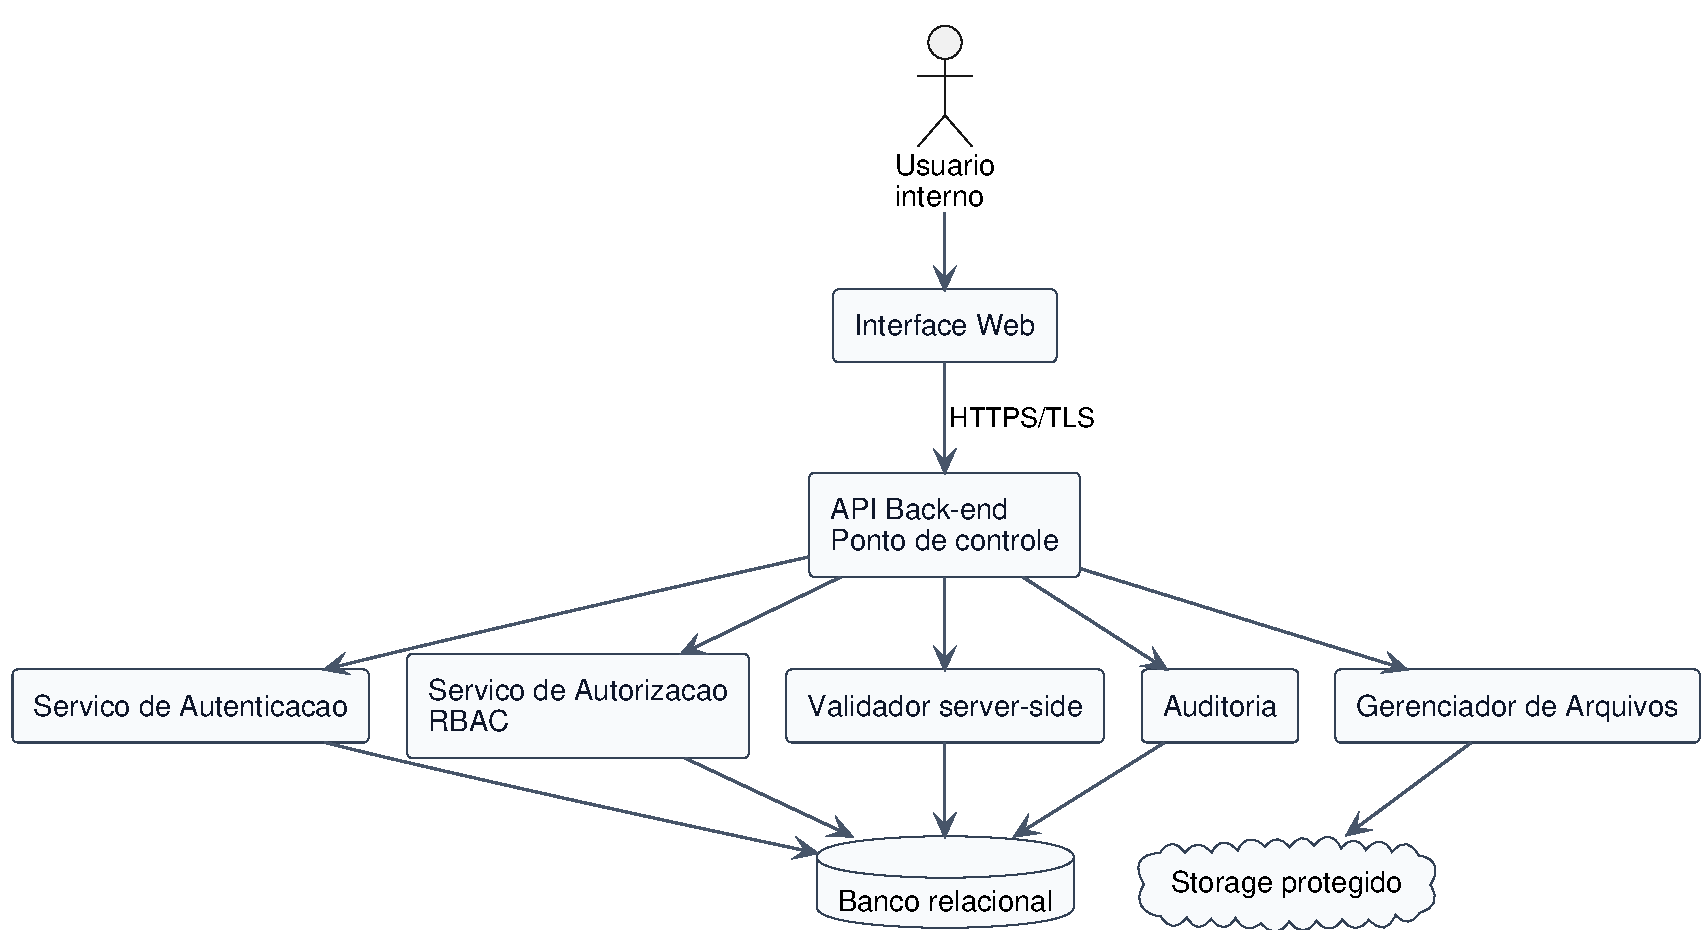
\includegraphics[width=0.85\textwidth,height=0.55\textheight,keepaspectratio]{Imagens/arquitetura/M-V6-01-seguranca}
\caption{Modelo M-V6-01 -- Controles de segurança e conformidade.}
\label{fig:m-v6-01-seguranca}
\end{figure}

%% ─────────────────────────────────────────────
\section{Correspondências e Regras de Consistência}

Seguindo a ISO 42010, as correspondências (\textit{correspondences}) explicitam as relações entre elementos de diferentes views, garantindo consistência interna da descrição arquitetural.

A \autoref{tab:correspondence-rules} define as regras de correspondência estabelecidas para o SGC.

\begin{table}[htbp]
\caption{Regras de correspondência arquitetural.}
\label{tab:correspondence-rules}
\centering
\small
\begin{tabularx}{\textwidth}{|l|X|}
\hline
\textbf{Regra} & \textbf{Definição} \\
\hline
CR-01 & Todo componente presente em V2 (Lógica) deve ter pelo menos um participante correspondente nos diagramas de sequência de V1 ou V3. \\
CR-02 & Todo módulo de domínio em V2 deve ter um contêiner correspondente no diagrama de implantação V5. \\
CR-03 & Todo fluxo com dados sensíveis de pacientes em V1 ou V3 deve passar pelo autorizacaoService documentado em V6. \\
CR-04 & Toda operação de escrita nos diagramas V1 e V3 deve incluir chamada ao auditoriaService. \\
\hline
\end{tabularx}
\end{table}

A \autoref{tab:correspondencias} instancia as correspondências identificadas entre os elementos das views.

\begin{table}[htbp]
\caption{Correspondências arquiteturais.}
\label{tab:correspondencias}
\centering
\small
\begin{tabularx}{\textwidth}{|l|l|l|X|}
\hline
\textbf{ID} & \textbf{Elemento em} & \textbf{Corresponde em} & \textbf{Elemento correspondente} \\
\hline
CO-01 & ConsultaController (V1) & V2 & Módulo Agenda e Atendimento \\
CO-02 & DispensacaoController (V3) & V2 & Módulo Farmácia Clínica e Prescrição \\
CO-03 & autorizacaoService (V1, V3) & V6 & Serviço de Autorização RBAC \\
CO-04 & auditoriaService (V1, V3) & V6 & Auditoria \\
CO-05 & consultaRepository (V1) & V5 & Contêiner back-end/API → Supabase PostgreSQL \\
CO-06 & dispensacaoRepository (V3) & V5 & Contêiner back-end/API → Supabase PostgreSQL \\
\hline
\end{tabularx}
\end{table}

\subsection{Conformidade com o ArchCaMo}

A \autoref{tab:conformidade-archcamo} avalia o grau de conformidade desta descrição arquitetural com os critérios do ArchCaMo.

\begin{table}[htbp]
\caption{Conformidade da descrição arquitetural com o ArchCaMo.}
\label{tab:conformidade-archcamo}
\centering
\small
\begin{tabularx}{\textwidth}{|l|X|c|}
\hline
\textbf{Critério} & \textbf{Evidência neste documento} & \textbf{Status} \\
\hline
Concerns identificados       & Tabela~\ref{tab:concerns-arquitetura}: 12 concerns explícitos & \checkmark \\
Stakeholders documentados    & Tabela~\ref{tab:stakeholders-arquitetura}: 11 stakeholders & \checkmark \\
Viewpoints definidos         & Tabela~\ref{tab:viewpoints-visoes}: 6 viewpoints & \checkmark \\
Views com modelos            & M-V1-01 a M-V6-01 & \checkmark \\
Correspondências explícitas  & Tabelas~\ref{tab:correspondence-rules} e~\ref{tab:correspondencias}: 4 regras e 6 correspondências & \checkmark \\
Decisões arquiteturais       & Tabela~\ref{tab:decisoes-arquiteturais}: 8 decisões & \checkmark \\
Rastreabilidade              & Tabela~\ref{tab:rastreabilidade}: concerns × views × modelos × decisões & \checkmark \\
Model kinds declarados       & Tabela~\ref{tab:viewpoints-visoes}: UML Sequence, Component e Deployment & \checkmark \\
Rationale documentado        & Seção~\ref{sec:rationale}: rationale de 5 decisões principais & \checkmark \\
Consistência verificada      & CR-01 a CR-04 verificadas pelas correspondências CO-01 a CO-06 & \checkmark \\
\hline
\end{tabularx}
\end{table}

%% ─────────────────────────────────────────────
\section{Decisões Arquiteturais e Rationale}

As decisões arquiteturais registram as escolhas de design significativas que moldaram a estrutura do SGC, juntamente com a justificativa (\textit{rationale}) e as alternativas consideradas. A \autoref{tab:decisoes-arquiteturais} sintetiza as principais decisões.

\begin{table}[htbp]
\caption{Decisões arquiteturais resumidas.}
\label{tab:decisoes-arquiteturais}
\centering
\small
\begin{tabularx}{\textwidth}{|l|X|l|}
\hline
\textbf{ID} & \textbf{Decisão} & \textbf{Concerns} \\
\hline
DA01 & Adotar arquitetura em camadas (Apresentação, API, Aplicação, Domínio, Persistência) & C7, C8, C11 \\
DA02 & Expor API REST com contrato OpenAPI/Swagger & C8, C9 \\
DA03 & Implementar controle de acesso via RBAC com papéis pré-definidos & C1, C6 \\
DA04 & Adotar persistência relacional gerenciada e storage separado para arquivos clínicos (concretizada via Supabase) & C3, C10, C12 \\
DA05 & Adotar interface web SPA responsiva para fluxos operacionais (concretizada via React) & C9, C2 \\
DA06 & Operações críticas encapsuladas em transações atômicas no banco & C4 \\
DA07 & Serviço de auditoria centralizado chamado por todos os controllers & C5, C6 \\
DA08 & Pipeline CI/CD automatizado com ambientes de produção e homologação & C12, C3 \\
\hline
\end{tabularx}
\end{table}

\subsection{Rationale das Decisões Principais}
\label{sec:rationale}

\textbf{DA01 -- Arquitetura em Camadas:} A separação em camadas distintas (Apresentação, API, Aplicação, Domínio e Persistência) promove alta coesão e baixo acoplamento, facilitando testes unitários e a evolução independente de cada camada. A alternativa de microserviços foi descartada pela complexidade operacional incompatível com o tamanho da equipe e o prazo do projeto.

\textbf{DA03 -- RBAC:} O controle de acesso baseado em papéis permite gerenciar permissões de forma centralizada e auditável, sem necessidade de lógica de autorização distribuída nos módulos. Essa abordagem atende diretamente ao C1 e ao C6 (LGPD), evitando exposição indevida de dados sensíveis de pacientes.

\textbf{DA04 -- Persistência Relacional Gerenciada:} Adotar um banco relacional gerenciado (PostgreSQL via Supabase) com storage separado para arquivos clínicos reduz a carga operacional de configuração de infraestrutura de dados, permitindo que a equipe foque nas regras de negócio. O suporte a transações ACID atende C4; o storage separado satisfaz C10 e C6 (arquivos de pacientes cifrados em repouso).

\textbf{DA06 -- Transações Atômicas:} Operações como agendamento e dispensação envolvem múltiplas escritas que devem ser indivisíveis. O uso de transações de banco de dados garante que, em caso de falha parcial, nenhum estado inconsistente seja persistido, satisfazendo C4.

\textbf{DA07 -- Auditoria Centralizada:}\ Centralizar o registro de auditoria em um serviço dedicado (\texttt{auditoriaService}) garante que nenhuma operação crítica escape do rastreamento, independentemente do módulo que a dispara. Isso simplifica a conformidade com LGPD e facilita investigações.

%% ─────────────────────────────────────────────
\section{Rastreabilidade entre Concerns, Views, Modelos e Decisões}

A \autoref{tab:rastreabilidade} apresenta a matriz de rastreabilidade que relaciona cada concern arquitetural às views, modelos e decisões que o endereçam, demonstrando a completude da descrição arquitetural.

\begin{table}[H]
\caption{Rastreabilidade entre concerns, stakeholders, views, modelos e decisões.}
\label{tab:rastreabilidade}
\centering
\small
\begin{tabularx}{\textwidth}{|l|X|l|l|l|}
\hline
\textbf{Concern} & \textbf{Stakeholders} & \textbf{Views} & \textbf{Modelos} & \textbf{Decisões} \\
\hline
C1  & S3, S9               & V1, V6     & M-V1-01, M-V6-01                    & DA03, DA07 \\
C2  & S4, S5, S10          & V3         & M-V3-01                             & DA02, DA05 \\
C3  & S8                   & V5         & M-V5-01                             & DA04, DA08 \\
C4  & S2, S4, S5, S6, S7   & V1, V3     & M-V1-01, M-V3-01                    & DA06       \\
C5  & S3, S6, S9, S11      & V1, V3, V6 & M-V1-01, M-V3-01, M-V6-01          & DA07       \\
C6  & S3, S9               & V6         & M-V6-01                             & DA03, DA07 \\
C7  & S1, S2               & V2, V4     & M-V2-01, M-V4-01                    & DA01       \\
C8  & S1, S2               & V2, V3, V4 & M-V2-01, M-V3-01, M-V4-01          & DA02       \\
C9  & S4, S5, S7, S10, S11 & V2         & M-V2-01                             & DA05, DA02 \\
C10 & S6, S7, S8           & V2, V5     & M-V2-01, M-V5-01                    & DA04       \\
C11 & S1, S2               & V4         & M-V4-01                             & DA01       \\
C12 & S8, S11              & V5         & M-V5-01                             & DA04, DA08 \\
\hline
\end{tabularx}
\end{table}